\documentclass{article}
\usepackage{arxiv}

\usepackage[utf8]{inputenc} % allow utf-8 input
\usepackage[math]{anttor}   % Antykwa torunska
\usepackage[T1]{fontenc}    % use 8-bit T1 fonts
\usepackage{hyperref}       % hyperlinks
\usepackage{url}            % simple URL typesetting
\usepackage{booktabs}       % professional-quality tables
\usepackage{amsfonts}       % blackboard math symbols
\usepackage{nicefrac}       % compact symbols for 1/2, etc.
\usepackage{microtype}      % microtypography
\usepackage{graphicx}       % adding figures
\usepackage{float}
\usepackage{plantuml}

\begin{document}
\title{Mobile application Bluetooth frame documentation}
\maketitle
\section{Bluetooth data format}

CANlink wireless series 3000 uses the RM Byte Command Protocol, which serves for bi-directional transparent CAN message transmission between the host and the CAN network. To transfer CAN message through Bluetooth it needs to be encoded into command frames with specific byte values.

\begin{figure}[H]
    \centering
    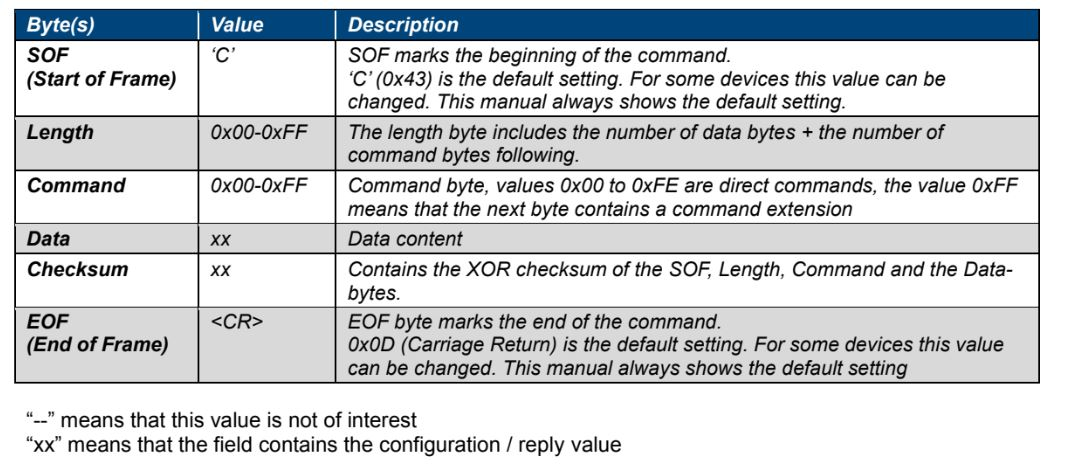
\includegraphics[width=\textwidth]{img/RM_Byte_Command.JPG}
    \label{fig:hs}
\end{figure}

% For more info refer to RM Byte Command Protocol manual available in the projects Dropbox.

\newpage
\section{Sensor data info Bluetooth frames}
% \subsection{Request data frame}
% From Mobile Application. This frame is used to ask robot to send its status frames.



\subsection{Engine frame 1}
From TTControl
\begin{itemize}
    \item Accumulator voltage (ACC\_VOL)
    \item Fuel Temperature (FT)
    \item Fuel Level (in litres) (FL)
    \item Engine Fuel Rate (EFR)
    \item Torque of engine (TRQ)
    \item Engine Rotations Per Minute (RPM)
\end{itemize}{}

\textbf{Frame length = 8 bytes}
\begin{center}
    \begin{tabular}{| p{20pt} | p{40pt} | p{40pt} | p{40pt} | p{40pt} | p{40pt} | p{40pt} | p{60pt} | p{60pt} |}
        \hline
        ID   & B0     & B1     & B2  & B3  & B4 & B5 & B6          & B7          \\
        \hline
        0x64 & RPM\_1 & RPM\_0 & TRQ & EFR & FL & FT & ACC\_VOL\_1 & ACC\_VOL\_0 \\
        \hline
    \end{tabular}

\end{center}

Decoding:
\begin{itemize}
    \item $ACC\_VOL = ((ACC\_VOL\_1<<8) | (ACC\_VOL\_0))/1000$
    \item $EFR = EFR/10$
\end{itemize}


\subsection{Engine frame 2}
From TTControl
\begin{itemize}
    \item ETH - engine total hours
    \item EFT - engine fuel total
\end{itemize}{}

\textbf{Frame length = 8 bytes}
\begin{center}
    \begin{tabular}{| p{20pt} | p{40pt} | p{40pt} | p{40pt} | p{40pt} | p{40pt} | p{40pt} | p{40pt} | p{40pt} |}
        \hline
        ID   & B0     & B1     & B2     & B3     & B4     & B5     & B6     & B7     \\
        \hline
        0x65 & ETH\_3 & ETH\_2 & ETH\_1 & ETH\_0 & EFT\_3 & EFT\_2 & EFT\_1 & EFT\_0 \\
        \hline
    \end{tabular}

\end{center}
Decoding:
\begin{itemize}
    \item $ETH = ((ETH\_1<<8) | (ETH\_0))/10$
    \item $EFT = ((EFT\_1<<8) | (EFT\_0))/10$
\end{itemize}

\subsection{Hydraulics data}
From TTControl
\begin{itemize}
    \item Momentary predicted work time with remaining fuel (WT)
    \item Hydraulic oil temperature (OT - usint)
    \item Hydraulic oil pressure (PRS)
\end{itemize}{}

\textbf{Frame length = 8 bytes}
\begin{center}
    \begin{tabular}{| p{20pt} | p{40pt} | p{40pt} | p{40pt} | p{40pt} | p{40pt} | p{40pt} | p{40pt} | p{40pt} |}
        \hline
        ID   & B0   & B1 & B2 & B3     & B4     & B5  & B6   & B7   \\
        \hline
        0x69 & 0xFF & WT & OT & PRS\_1 & PRS\_0 & RNG & 0xFF & 0xFF \\
        \hline
    \end{tabular}
\end{center}
Decoding:
\begin{itemize}
    \item $OT = OT - 80$
\end{itemize}

\subsection{Carts angle and chassis angle}
From TTControl
\begin{itemize}
    \item CR\_F - front cart rotation (CR=CR/10)
    \item CR\_B - back cart rotation (CR=CR/10)
    \item X axis inclinometer value (along Agribot chasis), (X\_INC=X\_INC/10)
    \item Y axis inclinometer value (along Agribot chasis), (Y\_INC=Y\_INC/10)
\end{itemize}{}

\textbf{Frame length = 8 bytes}
\begin{center}
    \begin{tabular}{| p{20pt} | p{40pt} | p{40pt} | p{40pt} | p{40pt} | p{40pt} | p{40pt} | p{40pt} | p{40pt} |}
        \hline
        ID   & B0     & B1     & B2     & B3     & B4        & B5        & B6        & B7        \\
        \hline
        0x6A & CRF\_1 & CRF\_0 & CRB\_1 & CRB\_0 & X\_INC\_1 & X\_INC\_0 & Y\_INC\_1 & Y\_INC\_0 \\
        \hline
    \end{tabular}

\end{center}
Decoding:
\begin{itemize}
    \item All above values needs to be devided by 10 (same maner as in ETH in Frame 2).
\end{itemize}


\newpage
\section{State changing and command frames}
\subsection{Heartbeat frame}
From Mobile Application and TTControl. This frame needs to be send with proper value at least every 500 ms or robot will terminate the connection with mobile application. The initial Heartbeat value (HB\_ID) of 0 is send by mobile application and then robot answers with the same value of HB\_ID, which is then incremented by the application and send back. Robot once again check if the HB\_ID is proper and send back the answer or breaks the connection if the value was bad. This process is repeated cyclically (at least every 200 ms), every 255 the HB\_ID rounds back at 0.

\textbf{Frame length = 1 byte}
\begin{center}
    \begin{tabular}{| p{20pt} | p{40pt} | p{40pt} | p{40pt} | p{40pt} | p{40pt} | p{40pt} | p{40pt} | p{40pt} |}
        \hline
        ID   & B0     & B1 & B2 & B3 & B4 & B5 & B6 & B7 \\
        \hline
        0x01 & HB\_ID & *  & *  & *  & *  & *  & *  & *  \\
        \hline
    \end{tabular}
\end{center}

\begin{plantuml}
    @startuml
    MobileApp -> MobileApp : value = 0
    MobileApp -> TTControl : HB_ID = value
    TTControl -> TTControl : Check if this is an initial value
    MobileApp <-- TTControl: HB_ID = value
    loop
        MobileApp -> MobileApp : Increment value
        MobileApp -> TTControl : HB_ID = value
        TTControl -> TTControl : Check if the difference between the received value the last one is equal to 1
        MobileApp <-- TTControl: HB_ID = value
    end
    @enduml
\end{plantuml}


\subsection{Handshake frame}
From Mobile Application. This frame initializes all the communication with the robot.

\textbf{Frame length = 1 byte}
\begin{center}
    \begin{tabular}{| p{20pt} | p{40pt} | p{40pt} | p{40pt} | p{40pt} | p{40pt} | p{40pt} | p{40pt} | p{40pt} |}
        \hline
        ID   & B0   & B1 & B2 & B3 & B4 & B5 & B6 & B7 \\
        \hline
        0x0A & 0x01 & *  & *  & *  & *  & *  & *  & *  \\
        \hline
    \end{tabular}
\end{center}

\textbf{Frame length = 1 byte}
\begin{center}
    \begin{tabular}{| p{20pt} | p{40pt} | p{40pt} | p{40pt} | p{40pt} | p{40pt} | p{40pt} | p{40pt} | p{40pt} |}
        \hline
        ID   & B0   & B1 & B2 & B3 & B4 & B5 & B6 & B7 \\
        \hline
        0x0B & 0x01 & *  & *  & *  & *  & *  & *  & *  \\
        \hline
    \end{tabular}
\end{center}

TTControl send the exact same message as the confirmation of receiving this command.

\begin{plantuml}
    @startuml
    MobileApp -> TTControl : ID = 0x0A
    MobileApp <-- TTControl: ID = 0x0B
    @enduml
\end{plantuml}

\subsection{Manual steering initialization}
From Mobile Application. The data is only one dummy byte. This frame is used to initiate the manual steering state.

\textbf{Frame length = 1 byte}
\begin{center}
    \begin{tabular}{| p{20pt} | p{40pt} | p{40pt} | p{40pt} | p{40pt} | p{40pt} | p{40pt} | p{40pt} | p{40pt} |}
        \hline
        ID   & B0   & B1 & B2 & B3 & B4 & B5 & B6 & B7 \\
        \hline
        0x14 & 0x14 & *  & *  & *  & *  & *  & *  & *  \\
        \hline
    \end{tabular}
\end{center}
TTControl send the exact same message as the confirmation of receiving this command.
\subsection{Manual steering ready}
From TTControl. The data is only one dummy byte. This frame is send to inform mobile application that the manual steering commands set is now active.

\textbf{Frame length = 1 byte}
\begin{center}
    \begin{tabular}{| p{20pt} | p{40pt} | p{40pt} | p{40pt} | p{40pt} | p{40pt} | p{40pt} | p{40pt} | p{40pt} |}
        \hline
        ID   & B0   & B1 & B2 & B3 & B4 & B5 & B6 & B7 \\
        \hline
        0x15 & 0x15 & *  & *  & *  & *  & *  & *  & *  \\
        \hline
    \end{tabular}
\end{center}

\begin{plantuml}
    @startuml
    MobileApp -> TTControl : ID = 0x14
    MobileApp <-- TTControl: ID = 0x14
    TTControl -> TTControl : MANUAL_READY
    MobileApp <-- TTControl : ID = 0x15
    MobileApp -> TTControl : ID = 0x15
    TTControl -> TTControl : MANUAL_ACTIVE
    @enduml
\end{plantuml}

\newpage
\section{Error frames}
\subsection{Error frames}
If the there is an error with robot, a frame describing the problem is send
\begin{itemize}
    \item ERR -- a 2-byte number describing error code
\end{itemize}{}

\textbf{Frame length = 2}
\begin{center}
    \begin{tabular}{| p{20pt} | p{40pt} | p{40pt} | p{40pt} | p{40pt} | p{40pt} | p{40pt} | p{40pt} | p{40pt} |}
        \hline
        ID   & B0     & B1     & B2 & B3 & B4 & B5 & B6 & B7 \\
        \hline
        0xC8 & ERR\_1 & ERR\_0 & *  & *  & *  & *  & *  & *  \\
        \hline
    \end{tabular}
\end{center}

\subsection{Engine error frames start}
If there are errors in the engine, a frame announcing the problem is send
\begin{itemize}
    \item ERR\_TOT -- a byte number describing total error count
    \item LAMP\_STATE -- the state of lamps which describe the severity of the problems
\end{itemize}{}

\textbf{Frame length = 2}
\begin{center}
    \begin{tabular}{| p{20pt} | p{45pt} | p{60pt} | p{40pt} | p{40pt} | p{40pt} | p{40pt} | p{40pt} | p{40pt} |}
        \hline
        ID    & B0       & B1          & B2 & B3 & B4 & B5 & B6 & B7 \\
        \hline
        0x104 & ERR\_TOT & LAMP\_STATE & *  & *  & *  & *  & *  & *  \\
        \hline
    \end{tabular}
\end{center}

\subsection{Engine error frames}
A frame containing one of the announced error frames. Byte order LSB first.
\begin{itemize}
    \item ERR\_NUM -- an number number, value up to the announced in Engine error frames start
    \item SPN -- the 3-byte error code described in Deutz documents
    \item FMI -- the error specific code described in Deutz documents
    \item OCC -- the error occurrence count
    \item ERR\_STATE -- if the error is active, contains 1, if passive 0
\end{itemize}{}

\textbf{Frame length = 8}
\begin{center}
    \begin{tabular}{| p{20pt} | p{45pt} | p{60pt} | p{40pt} | p{40pt} | p{40pt} | p{40pt} | p{55pt} | p{40pt} |}
        \hline
        ID    & B0       & B1     & B2     & B3     & B4  & B5  & B6         & B7   \\
        \hline
        0x105 & ERR\_NUM & SPN\_0 & SPN\_1 & SPN\_2 & FMI & OCC & ERR\_STATE & 0xFF \\
        \hline
    \end{tabular}
\end{center}

\subsection{Manual error frames}
If the there is an error during manual commands, an error frame is sent
\begin{itemize}
    \item ERR -- a 2-byte number describing error code
\end{itemize}{}

\textbf{Frame length = 2}
\begin{center}
    \begin{tabular}{| p{20pt} | p{40pt} | p{40pt} | p{40pt} | p{40pt} | p{40pt} | p{40pt} | p{40pt} | p{40pt} |}
        \hline
        ID   & B0     & B1     & B2 & B3 & B4 & B5 & B6 & B7 \\
        \hline
        0xC9 & ERR\_1 & ERR\_0 & *  & *  & *  & *  & *  & *  \\
        \hline
    \end{tabular}
\end{center}

\newpage
\section{Manual command frames}

\subsection{Override cart linear movement}

Mobile application to TTControl.

\begin{itemize}
    \item DIR - if 1, go forward, if 0, go backward
    \item CART\_VEL - velocity of cart (in old agribot default value was 0xFF)
    \item FRONT\_SEL - if 1, front cart selected. If 0, front cart deselected
    \item BACK\_SEL - if 1, back cart selected. If 0, back cart deselected
\end{itemize}{}

\textbf{Frame length = 4}
\begin{center}
    \begin{tabular}{|c| c | c | c | c | c | c | c | c |}
        \hline
        ID   & B0  & B1        & B2         & B3         & B4 & B5 & B6 & B7 \\
        \hline
        0x32 & DIR & CART\_VEL & FRONT\_SEL & FRONT\_SEL & *  & *  & *  & *  \\
        \hline
    \end{tabular}
\end{center}

\begin{plantuml}
    @startuml
    MobileApp -> TTControl : ID = 0x32, 
    MobileApp <-- TTControl: ID = 0x32, B0=0x32 (confirmation)
    @enduml
\end{plantuml}

\subsection{Override cart rotation}

Mobile application to TTControl.

\begin{itemize}
    \item CART\_FRONT - if 1, front cart is selected and will rotate, if 0, front cart will be ignored
    \item DIR\_FRONT - if 1, rotate front cart left, if 0, rotate front cart right
    \item CART\_BACK - if 1, back cart is selected and will rotate, if 0, back cart will be ignored
    \item DIR\_BACK - if 1, rotate back cart left, if 0, rotate back cart right
\end{itemize}{}

\textbf{Frame length = 4}
\begin{center}
    \begin{tabular}{|c| c | c | c | c | c | c | c | c |}
        \hline
        ID   & B0          & B1         & B2         & B3        & B4 & B5 & B6 & B7 \\
        \hline
        0x33 & CART\_FRONT & DIR\_FRONT & CART\_BACK & DIR\_BACK & *  & *  & *  & *  \\
        \hline
    \end{tabular}
\end{center}

\begin{plantuml}
    @startuml
    MobileApp -> TTControl : ID = 0x33, 
    MobileApp <-- TTControl: ID = 0x33, B0=0x33 (confirmation)
    @enduml
\end{plantuml}

\subsection{Joystick frame}
From Mobile Application. This frame is used to move the robot around and needs to be send every 300 ms or the command timeout will occur and the controller will halt the outputs and the robot will stop.
\begin{itemize}
    \item DIR\_V - velocity direction (negative velocity means forward movement, positive - backward movement)
    \item DIR\_R - radius direction (negative radius means right, positive - left)
    \item RAD - radius value
    \item VEL - velocity value
\end{itemize}{}

\textbf{Frame length = 8 }
\begin{center}
    \begin{tabular}{| p{20pt} | p{40pt} | p{40pt} | p{40pt} | p{40pt} | p{40pt} | p{40pt} | p{40pt} | p{40pt} |}
        \hline
        ID   & B0     & B1     & B2     & B3     & B4     & B5     & B6   & B7   \\
        \hline
        0x35 & DIR\_V & DIR\_R & RAD\_1 & RAD\_0 & VEL\_1 & VEL\_0 & 0xFF & 0xFF \\
        \hline
    \end{tabular}
\end{center}

Decoding:
\begin{itemize}
    \item $RAD = RAD/10$
    \item $VEL = VEL/100$
\end{itemize}


\subsection{Start Engine}
From Mobile Application. This frame is used to start the engine, by sending 2 of them in interval shorter than 200 ms and stop the engine by sending it for 2 seconds.

\textbf{Frame length = 1}
\begin{center}
    \begin{tabular}{| p{20pt} | p{40pt} | p{40pt} | p{40pt} | p{40pt} | p{40pt} | p{40pt} | p{40pt} | p{40pt} |}
        \hline
        ID   & B0   & B1 & B2 & B3 & B4 & B5 & B6 & B7 \\
        \hline
        0x5A & 0xFF & *  & *  & *  & *  & *  & *  & *  \\
        \hline
    \end{tabular}
\end{center}

\begin{plantuml}
    @startuml
    MobileApp -> TTControl : ID = 0xFF, B0=0xFF
    MobileApp -> TTControl : ID = 0x5A
    @enduml
\end{plantuml}


\subsection{STOP Engine}
From Mobile Application. This frame is used to stop any ongoing track moving tasks like, aligning carts and switches. It is used to start and stop the engine too, by sending first this frame and then an Start Stop engine frame.

\textbf{Frame length = 1 }
\begin{center}
    \begin{tabular}{| p{20pt} | p{40pt} | p{40pt} | p{40pt} | p{40pt} | p{40pt} | p{40pt} | p{40pt} | p{40pt} |}
        \hline
        ID   & B0   & B1 & B2 & B3 & B4 & B5 & B6 & B7 \\
        \hline
        0xFF & 0xFF & *  & *  & *  & *  & *  & *  & *  \\
        \hline
    \end{tabular}
\end{center}

\begin{plantuml}
    @startuml
    MobileApp -> TTControl : ID = 0xFF, B0=0xFF
    MobileApp -> TTControl : ID = 0x5A
    @enduml
\end{plantuml}

\subsection{Change front delta geometry}
From Mobile Application. This is a request frame used to put up or down front caterpillars.

\begin{itemize}
    \item REQ\_RES - a code number describing the meaning of the frame (request or response), in this case 0 (change request)
    \item CAT\_STA - caterpillar state, 0 for normal caterpillar state, 1 (anything but 0) for elevated caterpillar state
\end{itemize}{}

\textbf{Frame length = 2 bytes}
\begin{center}
    \begin{tabular}{| p{20pt} | p{40pt} | p{40pt} | p{40pt} | p{40pt} | p{40pt} | p{40pt} | p{40pt} | p{40pt} |}
        \hline
        ID   & B0   & B1 & B2 & B3 & B4 & B5 & B6 & B7 \\
        \hline
        0x1F5 & REQ\_RES & CAT\_STA  & *  & *  & *  & *  & *  & *  \\
        \hline
    \end{tabular}
\end{center}

From Advantech to Mobile Application. This frame is a callback from putting up or down front caterpillars.

\begin{itemize}
    \item REQ\_RES - a code number describing the meaning of the frame (request or response), in this case 1 (change response)
    \item CAT\_STA - caterpillar state, 0 for normal caterpillar state, 1 for elevated caterpillar state, 2 for unknown caterpillar state
\end{itemize}{}

\textbf{Frame length = 2 bytes}
\begin{center}
    \begin{tabular}{| p{20pt} | p{40pt} | p{40pt} | p{40pt} | p{40pt} | p{40pt} | p{40pt} | p{40pt} | p{40pt} |}
        \hline
        ID   & B0   & B1 & B2 & B3 & B4 & B5 & B6 & B7 \\
        \hline
        0x1F5 & REQ\_RES & CAT\_STA  & *  & *  & *  & *  & *  & *  \\
        \hline
    \end{tabular}
\end{center}

\subsection{Change back delta geometry}
From Mobile Application. This frame is used to put up or down back caterpillars.

\begin{itemize}
    \item REQ\_RES - a code number describing the meaning of the frame (request or response), in this case 0 (change request)
    \item CAT\_STA - caterpillar state, 0 for normal caterpillar state, 1 (anything but 0) for elevated caterpillar state
\end{itemize}{}

\textbf{Frame length = 2 bytes}
\begin{center}
    \begin{tabular}{| p{20pt} | p{40pt} | p{40pt} | p{40pt} | p{40pt} | p{40pt} | p{40pt} | p{40pt} | p{40pt} |}
        \hline
        ID   & B0   & B1 & B2 & B3 & B4 & B5 & B6 & B7 \\
        \hline
        0x1F5 & REQ\_RES & CAT\_STA  & *  & *  & *  & *  & *  & *  \\
        \hline
    \end{tabular}
\end{center}

From Advantech to Mobile Application. This frame is a callback from putting up or down back caterpillars.

\begin{itemize}
    \item REQ\_RES - a code number describing the meaning of the frame (request or response), in this case 1 (change response)
    \item CAT\_STA - caterpillar state, 0 for normal caterpillar state, 1 for elevated caterpillar state, 2 for unknown caterpillar state
\end{itemize}{}

\textbf{Frame length = 2 bytes}
\begin{center}
    \begin{tabular}{| p{20pt} | p{40pt} | p{40pt} | p{40pt} | p{40pt} | p{40pt} | p{40pt} | p{40pt} | p{40pt} |}
        \hline
        ID   & B0   & B1 & B2 & B3 & B4 & B5 & B6 & B7 \\
        \hline
        0x1F5 & REQ\_RES & CAT\_STA  & *  & *  & *  & *  & *  & *  \\
        \hline
    \end{tabular}
\end{center}

\newpage
\section{Tools control}

\subsection{Control tool override - controlling the valves}
From Mobile Application to TTControl (also from Advantech to TTControl). Every switch control a hydraulic valve connected to a specific part of the robot tools.
\subsubsection{Frame}
\begin{itemize}
    \item SW\_ID - switch ID number
    \item SW\_ON - the switch should be ON (1) or OFF (0)
    \item SW\_LV - velocity value a percent integer number from 0 to 100, numbers larger than 100 are treated as mistakes and the switch is instantly closed
\end{itemize}{}

\textbf{Frame length = 3}
\begin{center}
    \begin{tabular}{| p{20pt} | p{40pt} | p{40pt} | p{40pt} | p{40pt} | p{40pt} | p{40pt} | p{40pt} | p{40pt} |}
        \hline
        ID   & B0     & B1     & B2     & B3 & B4 & B5 & B6 & B7 \\
        \hline
        0x3C & SW\_ID & SW\_ON & SW\_LV & *  & *  & *  & *  & *  \\
        \hline
    \end{tabular}
\end{center}

\subsubsection{SW\_ID} \label{sw_id}
\begin{itemize}
    \item 0x00 - Config to all switches
    \item 0x01 - FRONT\_PTO
    \item 0x02 - FRONT\_RED
    \item 0x03 - FRONT\_GREEN
    \item 0x04 - FRONT\_BLUE
    \item 0x05 - FRONT\_TPL\_ANGLE
    \item 0x06 - FRONT\_TPL\_HEIGHT
    \item 0x07 - BACK\_PTO
    \item 0x08 - BACK\_RED
    \item 0x09 - BACK\_GREEN
    \item 0x0A - BACK\_BLUE
    \item 0x0B - BACK\_TPL\_ANGLE
    \item 0x0C - BACK\_TPL\_HEIGHT
\end{itemize}

In return TTControl sends back confirmation frame:

\textbf{Frame length = 1}
\begin{center}
    \begin{tabular}{| p{20pt} | p{40pt} | p{40pt} | p{40pt} | p{40pt} | p{40pt} | p{40pt} | p{40pt} | p{40pt} |}
        \hline
        ID   & B0   & B1 & B2 & B3 & B4 & B5 & B6 & B7 \\
        \hline
        0x3C & 0x3C & *  & *  & *  & *  & *  & *  & *  \\
        \hline
    \end{tabular}
\end{center}

\subsection{Control tool position - manual mode steering}
From Mobile Application to Advantech. In this case, the destination configuration of tool is sent via the CAN frame. The units inside the frame differs depending on SW\_ID. Details are listed in below subsections.
\subsubsection{Frame - set TPL position - request}
\begin{itemize}
    \item CONF\_ID - config ID number (IDs are identical to those listed in section [\ref{sw_id}])
    \item CONF\_VAL\_Bx - values specific to ID
\end{itemize}{}

\textbf{Frame length = 3}
\begin{center}
    \begin{tabular}{| p{30pt} | p{45pt} | p{70pt} | p{70pt} | p{40pt} | p{40pt} | p{40pt} | p{40pt} | p{40pt} |}
        \hline
        ID    & B0       & B1            & B2            & B3 & B4 & B5 & B6 & B7 \\
        \hline
        0x13D & CONF\_ID & CONF\_VAL\_B1 & CONF\_VAL\_B0 & *  & *  & *  & *  & *  \\
        \hline
    \end{tabular}
\end{center}

\subsubsection{Frame - set TPL position response}
From Advantech to Mobile app.
\begin{itemize}
    \item CONF\_ID - config ID number (IDs are identical to those listed in section [\ref{sw_id}])
    \item RET - 0xFF - failed to set TPL config (for instance values are out of range); 0x00 - successfully set TPL config
\end{itemize}{}

\textbf{Frame length = 2}
\begin{center}
    \begin{tabular}{| p{30pt} | p{45pt} | p{70pt} | p{70pt} | p{40pt} | p{40pt} | p{40pt} | p{40pt} | p{40pt} |}
        \hline
        ID    & B0       & B1  & B2 & B3 & B4 & B5 & B6 & B7 \\
        \hline
        0x13E & CONF\_ID & RET & *  & *  & *  & *  & *  & *  \\
        \hline
    \end{tabular}
\end{center}



\subsubsection{CONF\_VAL\_Bx units and frame decoding}
\begin{itemize}
    \item FRONT\_PTO\textbackslash BACK\_PTO - rotations per minute. Range from 0 RPM to 1000 RPM. The value in the frame is delivered on two bytes. The value can be calculated using following formula:

          $VAL = (CONF\_VAL\_B1<<8) | (CONF\_VAL\_B0)$
    \item FRONT\_GREEN\textbackslash BACK\_GREEN - valve flow control. Range from 0 to 100\%.

          $VAL = (CONF\_VAL\_B0)$
    \item FRONT\_YELLOW\textbackslash BACK\_YELLOW - valve flow control. Range from 0 to 100\%.

          $VAL = (CONF\_VAL\_B0)$
    \item FRONT\_BLUE\textbackslash BACK\_BLUE - valve flow from 0 to 100.

          $VAL = (CONF\_VAL\_B0)$
    \item FRONT\_TPL\_ANGLE\textbackslash BACK\_TPL\_ANGLE - radians (from -0.26rad to 0.52rad). The negative number can be achieved by setting the highest bit to 1 in CONF\_VAL\_B1. The decoding can be performed by extracting sign bit, then setting the sign bit to 0. The resulding number should be devided by 1000.

          Example decoding: 0x8521. The 0x80 is indicates that the number is negative. We set the highest bit to 0. 0x0521 in hex is 1313. We divide the number by 1000 and multiply the number by -1. The result is -0.1313
    \item FRONT\_TPL\_HEIGHT\textbackslash BACK\_TPL\_HEIGHT - ejection of prismatic joint (from 0.0m to 0.45m). The decoding process is analogous to to angle frame, but without the sign
\end{itemize}

\subsection{TPL position feedback}

Frame send periodically from Advantech to Mobile app. Feedback from sensors mounted on robot.

\begin{itemize}
    \item CONF\_ID - config ID number (IDs are identical to those listed in section [\ref{sw_id}])
    \item CONF\_VAL\_Bx - values specific to ID
\end{itemize}{}

\textbf{Frame length = 3}
\begin{center}
    \begin{tabular}{| p{30pt} | p{45pt} | p{70pt} | p{70pt} | p{40pt} | p{40pt} | p{40pt} | p{40pt} | p{40pt} |}
        \hline
        ID    & B0       & B1            & B2            & B3 & B4 & B5 & B6 & B7 \\
        \hline
        0x13F & CONF\_ID & CONF\_VAL\_B1 & CONF\_VAL\_B0 & *  & *  & *  & *  & *  \\
        \hline
    \end{tabular}
\end{center}

\newpage
\section{RFID frames}

\subsection{Trigger scan} \label{trigger_scan}
From mobile application to Advantech. The frame triggers scan from selected antenna.

\begin{itemize}
    \item COM -- a code number describing the meaning of the frame, in this case 1 (scan request)
    \item ANT\_SEL -- 0x01 - front antenna selected, 0x02 - back antenna selected, 0x03 - both antennas selected
\end{itemize}{}

\textbf{Frame length = 2}
\begin{center}
    \begin{tabular}{| p{20pt} | p{40pt} | p{55pt} | p{55pt} | p{40pt} | p{40pt} | p{40pt} | p{40pt} | p{40pt} |}
        \hline
        ID    & B0  & B1       & B2 & B3 & B4 & B5 & B6 & B7 \\
        \hline
        0x1F4 & COM & ANT\_SEL & *  & *  & *  & *  & *  & *  \\
        \hline
    \end{tabular}
\end{center}

\subsection{Detected tags - response}
From Advantech to mobile application. In reply to trigger scan frame [\ref{trigger_scan}], the tags ID are sent. The EPC can be long up to 496 bits. In following example, the EPC tag is 9 bytes long.

\begin{itemize}
    \item COM -- a code number describing the meaning of the frame, in this case 2 (scan response start)
    \item TAG\_ANT -- 0x01 - tag detected by front antenna, 0x02 - tag detected by back antenna
    \item TAG\_LEN -- numbers of bytes
    \item TAG\_ID -- a 2-byte number representing the RFID tag ID
\end{itemize}{}

\textbf{Frame length = 3}
\begin{center}
    \begin{tabular}{| p{20pt} | p{45pt} | p{55pt} | p{55pt} | p{55pt} | p{55pt} | p{40pt} | p{40pt} | p{40pt} |}
        \hline
        ID    & B0  & B1       & B2       & B3 & B4 & B5 & B6 & B7 \\
        \hline
        0x1F4 & COM & TAG\_ANT & TAG\_LEN & *  & *  & *  & *  & *  \\
        \hline
    \end{tabular}
\end{center}

\textbf{Frame length = 8}

\begin{itemize}
    \item COM -- a code number describing the meaning of the frame, in this case 3 (scan response tag data pt 1)
\end{itemize}

\begin{center}
    \begin{tabular}{| p{20pt} | p{20pt} | p{50pt} | p{50pt} | p{50pt} | p{50pt} | p{50pt} | p{50pt} | p{50pt} |}
        \hline
        ID    & B0  & B1          & B2          & B3          & B4          & B5          & B6          & B7          \\
        \hline
        0x1F4 & COM & TAG\_ID\_B0 & TAG\_ID\_B1 & TAG\_ID\_B2 & TAG\_ID\_B3 & TAG\_ID\_B4 & TAG\_ID\_B5 & TAG\_ID\_B6 \\
        \hline
    \end{tabular}
\end{center}

\textbf{Frame length = 8}

If the ID is larger than capacity of frame, COM will increment.

\begin{itemize}
    \item COM -- a code number describing the meaning of the frame, in this case 4 (scan response tag data pt 2)
\end{itemize}

\begin{center}
    \begin{tabular}{| p{20pt} | p{20pt} | p{50pt} | p{50pt} | p{50pt} | p{50pt} | p{50pt} | p{50pt} | p{50pt} |}
        \hline
        ID    & B0  & B1          & B2          & B3   & B4   & B5   & B6   & B7   \\
        \hline
        0x1F4 & COM & TAG\_ID\_B8 & TAG\_ID\_B9 & 0x00 & 0x00 & 0x00 & 0x00 & 0x00
        \\
        \hline
    \end{tabular}
\end{center}


\end{document}
